
\documentclass[12pt]{amsart}
\usepackage{graphicx}
\usepackage{geometry} % see geometry.pdf on how to lay out the page. There's lots.
\usepackage[utf8]{inputenc}
\geometry{a4paper} % or letter or a5paper or ... etc

% \geometry{landscape} % rotated page geometry

% See the ``Article customise'' template for come common customisations

\title{Übersetzer Projekt}
%\subtitle{Impro-3 (Applied Textmining)}
\author{Christoph Brücke \\
	Christian Fischer\\
	Robert Schulz}
\date{} % delete this line to display the current date

%%% BEGIN DOCUMENT
\begin{document}

\maketitle
\tableofcontents

\section{Wort-für-Wort Übersetzer}
\subsection{Funktionsbeschreibung aller Komponenten}
Die Translator-Klasse ist der Haupteinstiegspunkt. Sie verbindet das Dictionary mit dem Language Model. Das angegebene Dictionary wird benutzt um eine Menge von Übersetzungen für ein gegebenes Wort zu erzeugen. Mit Hilfe des Language Models wird dann die passendste Übersetzung ausgewählt.\\
Die HashDictionary-Klasse ist eine Implementierung des Dictionary-Interfaces. Es kann mit einem DictionaryFileReader initialisiert werden. Aus einer Datei (zur Zeit nutzen wir das Dictionary von dict.cc) werden Übersetzungen gewonnen, die dann von der Translator-Klasse genutzt werden. Mit den addWord-Methoden werden Übersetzungen zum Dictionary hinzugefügt. Die translateWord- und translateSentence-Methoden liefern dann zu einem gegebenen (deutschen) Wort eine Menge von möglichen Übersetzungen.\\
Die BiGramModel-Klasse ist eine Implementierung des LanguageModel-Interfaces. Sie kann mit einem BufferedReader initialisiert werden mit dem dann aus einer Datei ein Textcorpus geladen wird, mit dem dann das Language Model trainiert wird. Mit den train-Methoden kann man mit einer Datei das Language Model trainieren oder aber mit Collection von String-Listen. Zur Zeit nutzen wir Protokolle des Europäischen Parlaments, aber der Corpus kann leicht ausgetauscht werden, je nach zu übersetzenden Text sogar mit einem, der speziell auf den gegebenen Kontext zugeschnitten ist. Mit der addUniGram-Methode werdendie Worte des Corpus zum Language Model hinzugefügt. Die addBiGram-Methode dagegen wird benutzt, um Worte, die im Text zusammenstehen, zum Language Model hinzuzufügen. Die getCount-Methoden geben die Anzahl der Vorkommen eines Wortes bzw. eines Wortpaares im Corpus wieder. Die UniGramProbability-Methode gibt die Wahrscheinlichkeit zurück, dass ein zufällig gewähltes Wort aus dem Corpus das gewählte ist. Die getBiGramProbability-Methode gibt zu einem gegeben Wortpaar die Wahrscheinlichkeit zurück, mit der das zweite Wort auf das erste folgt und nicht etwa ein anderes. So können aus einer Menge von Übersetzungen geeignete von ungeeigneten in den meisten Fällen getrennt werden.\\
Die ElcombriReader-Klasse ist eine Implementierung des DictionaryFileReader-Interfaces. Mit mehreren regulären Ausdrücken wird aus der Datei, deren Pfad dem ElcombriReader übergeben wird, ein DictionaryEntry für jeden Treffer erzeugt.\\
Die DictionaryEntry-Klasse steht für eine Datenstruktur, die einen Eintrag im Wörterbuch repräsentiert und die Daten für die Übersetzung bereithält.\\
\\
Das folgende UML-Klassendiagramm veranschaulicht die Zusammenhänge der Teile des Übersetzers.\\
\\
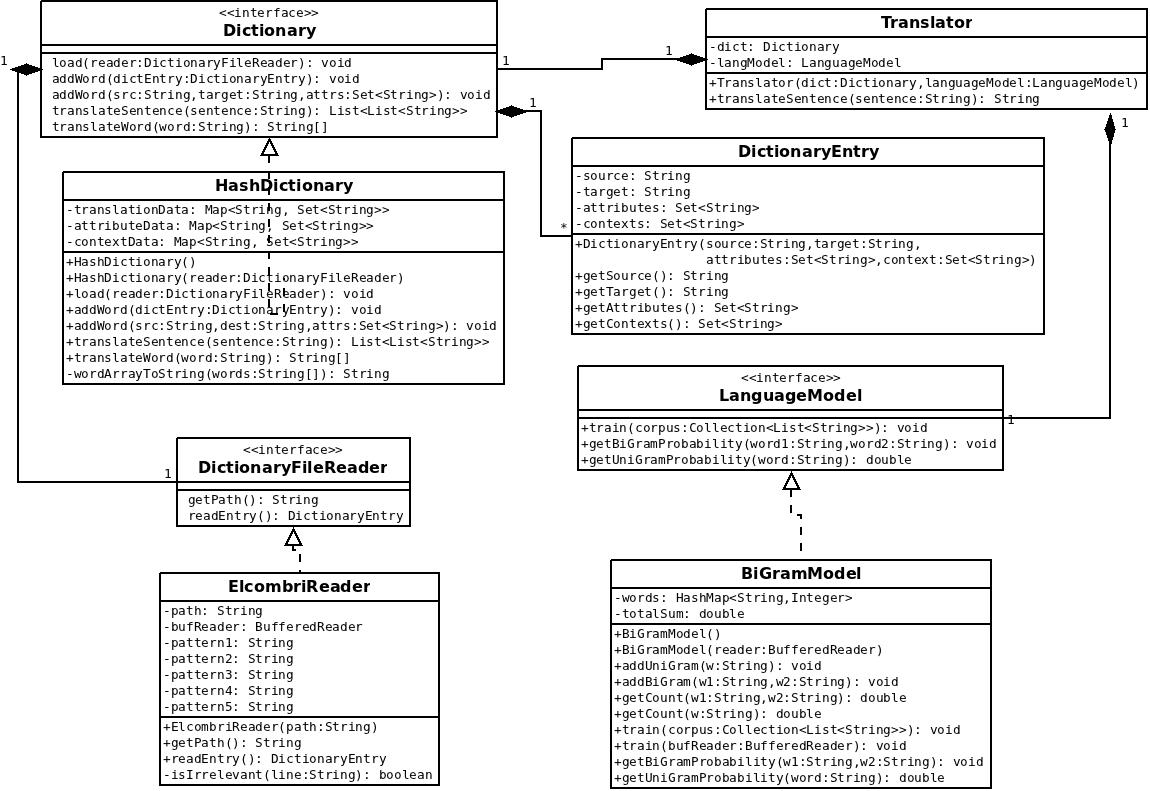
\includegraphics[scale=0.6,angle=90]{UML.jpg}

\subsection{Übersicht der Arbeitsaufteilung}
\vspace{\baselineskip}
Translator: Christian, Christoph, Robert\\
Dictionary/HashDictionary: Christian, Christoph, Robert\\
DictionaryEntry: Christian, Christoph, Robert\\
Language Model/BiGramModel: Christian\\
DictionaryFileReader/ElcombriReader: Robert
\end{document}
